\chapter{Вступ}

\section{Системна інженерія та верифікація}

    Протягом історії обчислювальної техніки було створено різні класи та способи обчислень,
    різні тоеорії та підходи до програмування таких систем, різні класи систем програмування.
    Зараз уже стало зрозумілим, що інженіринг систем які не піддаються до верифікації
    формальними методами не може бути застосований у галузях де вимоги до якості
    особливо підвищені, як то космонавтика, енергетика та фінанси.

    \paragraph{}
    Об'єктом дослідження данної роботи є системи верифікації програмного забезпечення
    та операційні системи яки виконують обчислення в реальному часі, їх поєднання
    та побудова формальної системи для унифікованого середовища, яке поєднує
    середовище виконання та систему верифікації у єдину систему мов.

    \paragraph{}
    Предметом дослідження такої системи мов є теорія типів, яка вивчає обчислювальні властивості мов.
    Теорія типів виділилася в окрему науку Мартіном Льофом як запит на ваканте місце у
    трикутнику теорій, які відповідають ізоморфізму Каррі-Говарда (Логіки, Мови, Категорії).
    Інші дві це: теорія категорій та логіка вищих порядків. Сама система доведення теорем є
    логікою, або аспектом логіки у трикутнику. Імплементація мови програмування,
    яка релізує логічну семантику здійснюється завдяки теорії типів. Формалізація методів
    відбувається завдяки теорії категорій, яка є абстрактною алгеброю фунцій,
    метематичним інструментом для формалізації мов програмування та довільних
    математичних теорій які описуються логіками вищих порядків.

\newpage
\section{Історія систем верифікації}

    \paragraph{}
    Перші спроби пошуку формального фундаменту для теорії обчислень були покладені
    Алонзо Черчем та Хаскелем Каррі у 30-х роках 20-го століття. Було запропоноване
    лямбда числення як апарат який може замінити класичну теорію множин та її аксіоматику,
    пропонуючи при цьому обчислювальну семантику. Пізніше в 1958, ця мова була втілена
    у вигляді LISP лауреатом премії тюрінга Джоном МакКарті, який працював в Прінстоні.
    Ця мова була побудована на таких примітивах, як: cons, nil, eq, atom, car, cdr,
    lambda, apply and id. Направді це уривки індуктивних конструкцій які були
    структуровані пізніше і формалізовані за допомогою теорії категорій Вільяма Лавіра.
    До цих пір нетипізоване лямбла числення є одною з мов у які робиться екстракт
    з сучасних пруверів. Окрім LISP, нетипізоване лямбда числення маніфестується у такі
    мови як Erlang, JavaScript, Python.

    \paragraph{}
    Перший математичний прувер AUTOMATH (і його модифікації AUT-68 та AUT-QE),
    який був написаний для комп'ютерів розроблявся під керівництвом де Брейна, 1967.
    У цьому прувері був квантор загальності та лямбда функція, таким чином це був перший прувер
    побудрваний на засадах ізоморфізма Каррі-Говарда.

    \paragraph{}
    ML/LCF або метамова і логіка обчисльювальних функцій був наступник крок до
    осягнення фундаментальної мови простору, тут впреше з'явилися алебраїчні типи даних
    у вигляді індуктивних типів, поліноміальних функторів або терміновані (well-founded) дерев.
    Пізніше були побувані категорні моделі Татсоя Хагіно (CPL) то Крокетом (Charity).
    Роберт Мілнер, асистований Морісом та Н'юві розробив Метамову (ML), як
    інструмент для побудови прувера LCF. LCF був основоположником у родині пруверів
    HOL88, HOL90, HOL98 та останньої версії на даний час HOL/Isabell.

    \paragraph{}
    У 80-90 роках були створені інші системи автоматичного доведення теорем,
    такі як Mizar (Трибулєк, 1989). PVS (Оур, Рушбі, Шанкар, 1995),
    ACL2 на базі Common Lisp (Боєр, Кауфман, Мур, 1996), Otter (МакКюн, 1996).


\newpage
\section{Методи верифікації}

    \paragraph{}
    Можна виділити два підходи до верифікації. Перший застосовується де вже є
    певна програма написана на певній мові програмування і потрібно довести ізоморфність
    цієї програми до доведеної моделі. Ця задача вирішується у побудові теоретичної моделі
    для певної мови програмування, потім програма на цій мові переводиться у цю
    теоретичну модель і доводить ізоморфізм цієї програми у побудованій моделі до доведеної моделі.
    Приклади таких систем та піходів. VST (CompCert, сертифікація Сі-програм),
    NuPRL (Cornell University, розподілені системи, залежні типи),
    TLA+ (Microsoft Reseach, Леслі Лампорт), Twelf (для верифікації мов програмування).

    \paragraph{}
    Інший підхід можна назвати підходом вбудованих DSL. Усе моделювання відбувається
    в основній мові, а сертифіковані програми автоматично екстрактяться в довільні мови.
    Приклади таких систем: Coq побудована на мові OCaml від науково-дослідного
    інституту Франції INRIA; Agda побудовані на мові Haskell від шведського інституту технологій Чалмерс;
    Lean побудована на мові C++ від Microsoft Research та Універсистету Каргені-Мелона;
    Idris подудована на мові Haskell Едвіна Бреді з шотландського Університету ім. св. Андрія;
    F* -- окремий проект Microsoft Research.

    \paragraph{}
    Завдання цього дослідження є побудова єдиної системи, яка поєднує середовище
    викодання та систему верифікації програмного забезпечення. Це прикладне дослідження,
    яке є фьюжином фундаментальної математики та інженерних систем з формальними методами верицікації.
    Методи цього дослідження є суто теоретичними.

\newpage
\section{Метематичне забезпечення}
\vspace{0.3cm}

\subsection{Теорія категорій}

    \paragraph{}
    Теорія категорій широко застосовується як інструмент для математиків у тому числі і
    при аналізі програмного забезпечення. Теорію категорій можна вважати абстрактною алгеброю функцій.
    Дамо конструктивне визначення категорії.
    Категорії (програми) визначаються переліком своїх об’єктів (типів) та своїх
    морфізмів (функцій), а також бінарною операцією композиції,
    що задовольняє закону асоціативності, та з тотожнім морфізмом (тотжньою функцією --- одиницею) який існує
    для кожного об’єкту (типу) категорії. Аксіоми формації об’єктів не
    приводяться та авто-постулуються в нижніх аксіомах. Аксіома формації
    морфізмів буде даватися як введеня експоненти після визначення декартового добутку.
    Поки що тут буде визначатися тільки композиція морфізмів. Об’єкти $A$ та $B$ морфізма $f: A \rightarrow B$
    називаються домен та кодомен відповідно.

    \paragraph{}
    Інтро аксіоми -- асоціативність композиції та права і ліва композиції одниці показують,
    що категорії є типизованими моноїдами, що складаються з морфізмів та операції композиції.
    Є різні мови, у тому числі і графічні, представлення категорної семантики, однак у цій роботі
    ми будемо використовувати теоретико-логічні формулювання.


\begin{fullwidth}[width=\linewidth+3cm]
\begingroup
\parbox[t][][l]{0.60\textwidth}{

\begin{prooftree}
\AxiomC{$\Gamma\ \vdash f: A \rightarrow B$ }
\AxiomC{$\Gamma\ \vdash g: B \rightarrow C$ }
\BinaryInfC{$\Gamma \vdash g \circ f : A \rightarrow C $}
\end{prooftree}

\begin{prooftree}
\AxiomC{$\Gamma \vdash f : B \rightarrow A$ }
\AxiomC{$\Gamma \vdash g : C \rightarrow B$ }
\AxiomC{$\Gamma \vdash h : D \rightarrow C$ }
\TrinaryInfC{$\Gamma \vdash (f \circ g) \circ h = f \circ (g \circ h) : D \rightarrow A $}
\end{prooftree}

}
\hspace{0.1cm}
\parbox[t][][r]{0.40\textwidth}{

\begin{prooftree}
\AxiomC{$$ }
\UnaryInfC{$\Gamma \vdash id_A : A \rightarrow A $}
\end{prooftree}

\begin{prooftree}
\AxiomC{$\Gamma\ \vdash f: A \rightarrow B$ }
\UnaryInfC{$\Gamma \vdash f \circ id_A = f : A \rightarrow B$}
\end{prooftree}

\begin{prooftree}
\AxiomC{$\Gamma\ \vdash f: A \rightarrow B$ }
\UnaryInfC{$\Gamma \vdash id_B \circ f = f : A \rightarrow B $}
\end{prooftree}

}
\endgroup

\end{fullwidth}

\newpage
    \paragraph{}
    Композиція показує можливість звязувати область значень попереднього обчислення (кодомен)
    та область визначення наступного обчислення (домен). Композиція є фундаментальною властивістю морфізмів.

\paragraph{}
\begin{tabular}{lll}
$1.$ & $A: *$\\
$2.$ & $A: *\ ,\ B: * \implies f: A \rightarrow B$\\
$3.$ & $f: B \rightarrow C\ ,\ g: A \rightarrow B \implies f \circ g : A \rightarrow C$\\
$4.$ & $(f \circ g) \circ h = f \circ (g \circ h)$\\
$5.$ & $A \implies id : A \rightarrow A$\\
$6.$ & $f \circ id = f$\\
$7.$ & $id \circ f = f$\\
\end{tabular}

\newpage
\subsection{Алгебраїчні типи даних}

    Після операції композиції, як способу конструювання нових об’єктів
    за допомогою морфізмів далі йде операція конструювання добутка двох об’єктів певної категорії,
    разом з добутком морфізмів зі спільним доменом, необхідних для визначення декартового добутка $A \times B$.

    \paragraph{}
    Це є внутрішня мова декартової категорії, у якій для будь яких двох доменів існує їх декартова сума (кодобутку)
    та декартовий добуток (косума, кортеж), за допомогою яких конструюються суми-протоколи та добутки-повідмоення,
    а також існує $\bot$ тип-термінал, та $\top$ тип-котермінал. Термінальними типами зручно термінувати рекурсивні
    типи даних, такі як списки. Ми будемо розглядати тільки категорії які маються добутки та суми.

    \paragraph{}
    Добуток має природні елімінатори $\pi$ зі спільним доменом, які є морфізмами-проекціями об’єктів добутка. Сума має оберненені
    елімінатори $\sigma$ зі спільним кодоменом. Як видно добуток є дуальний до суми з точністю до направлення стрілок,
    таким чином елімінатори $\pi$ та $\sigma$ є оберненими, тобто $\pi \circ \sigma = \sigma \circ \pi = id$.

\begin{fullwidth}[width=\linewidth+2cm]
\hspace{1cm}
\begingroup
\parbox[t][][l]{0.40\textwidth}{

\begin{prooftree}
\AxiomC{$\Gamma\ x: A \times B$ }
\UnaryInfC{$\Gamma \vdash \pi_1\ : A \times B \rightarrow A$;
           $\Gamma \vdash \pi_2\ : A \times B \rightarrow B$}
\end{prooftree}

\begin{prooftree}
\AxiomC{$\Gamma \vdash\  a:A$ }
\AxiomC{$\Gamma \vdash\  b:B$ }
\BinaryInfC{$\Gamma \vdash\ (a,b) : A \times B$ }
\end{prooftree}

\begin{prooftree}
\AxiomC{}
\UnaryInfC{$\Gamma \vdash\ \bot$ }
\end{prooftree}

}
\hspace{0cm}
\parbox[t][][r]{0.60\textwidth}{

\begin{prooftree}
\AxiomC{}
\UnaryInfC{$\Gamma \vdash\ \top$ }
\end{prooftree}

\begin{prooftree}
\AxiomC{$\Gamma \vdash\  a:A$ }
\AxiomC{$\Gamma \vdash\  b:B$ }
\BinaryInfC{$\Gamma\vdash a\ |\ b : A \otimes B$}
\end{prooftree}

\begin{prooftree}
\AxiomC{$\Gamma\ x: A \otimes B$ }
\UnaryInfC{$\Gamma \vdash \sigma_1: A \rightarrow A \otimes B$;
           $\Gamma \vdash \sigma_2: B \rightarrow A \otimes B$}
\end{prooftree}

}
\endgroup
\end{fullwidth}

    \paragraph{}
    Також додамо тут аксіому множення морфізмів, яка
    випливає з визначення добутка, яка необхідна для
    забезпечення аплікативного програмування.

\begin{prooftree}
\AxiomC{$\Gamma \vdash\ f:A \rightarrow B$ }
\AxiomC{$\Gamma \vdash\ g:A \rightarrow C$ }
\AxiomC{$\Gamma \vdash\ B \times C$ }
\TrinaryInfC{$\Gamma \vdash\ \langle f,g \rangle : A \rightarrow B \times C$ }
\end{prooftree}

\begin{center}
%$(f \circ g) \circ h = f \circ (g \circ h)$\\
%$f \circ id = f$\\
%$id \circ f = f$\\
$\pi_1 \circ \langle f, g \rangle = f$\\
$\pi_2 \circ \langle f, g \rangle = g$\\
$\langle f \circ \pi_1, f \circ \pi_2 \rangle = f$\\
$\langle f, g \rangle \circ h = \langle f \circ h, g \circ h \rangle$\\
$\langle \pi_1, \pi_2 \rangle = id$\\
\end{center}

\newpage

    \subsection{Лямбда числення}
    Будучи внутрішньою мовою декартово-замкненої категорії лямбда числення окрім змінних
    та констант у вигляді термів пропонує операції абстракції та аплікації, що визначає
    достатньо лаконічну та потужну структуру обчислень з функціями вищих порядків,
    та метатипизаціями, такими як System F, яка була запропонована
    вперше Робіном Мілнером в мові ML, та зараз присутня в більш складних,
    таких як System F$\omega$, системах Haskell та Scala.

    \paragraph{}
    Щоб пояснити функції з категоріальнї точки зору потрібно пояснити категоріальні
    експоненти $f : A^B$,  які є аналогами фукціональних просторів $f: A \rightarrow B$.
    Так як ми вже визначили добутки та термінали, то ми можемо визначити і експоненти,
    опускаючи усі категоріальні подробиці ми визначимо конструювання функції (операція абстракції),
    яка параметризується змінною $x$ у середовищі $\Gamma$; та її елімінатора -- операції аплікації
    функції до аргументу. Так визначаєьтся декартово-замкнена категорія.
    Визначається також рекурсивний механізм виклику функції
    з довільною кількістю аргументів.

\begin{fullwidth}
\hspace{-2cm}
\begingroup
\parbox[t][][l]{0.40\textwidth}{

\begin{prooftree}
\AxiomC{$\Gamma  x:A \vdash M : B$}
\UnaryInfC{$\Gamma \vdash \lambda\ x\ .\ M : A \rightarrow B$}
\end{prooftree}

\begin{prooftree}
\AxiomC{$\Gamma\ f:A \rightarrow B$ }
\AxiomC{$\Gamma\ a:A$ }
\BinaryInfC{$\Gamma \vdash apply\ f\ a\ : (A \rightarrow B) \times A \rightarrow B$}
\end{prooftree}

\begin{prooftree}
\AxiomC{$\Gamma \vdash f: A \times B \rightarrow C$ }
\UnaryInfC{$\Gamma \vdash curry\ f : A \rightarrow (B \rightarrow C)$}
\end{prooftree}

}
\hspace{1cm}
\parbox[t][][r]{0.60\textwidth}{

\begin{center}
$apply \circ \langle (curry\ f) \circ \pi_1 , \pi_2 \rangle = f$\\
$curry\ apply \circ \langle g \circ \pi_1, \pi_2 \rangle) = g$\\
$apply \circ \langle curry\ f, g \rangle = f \circ \langle id , g\rangle$\\
$(curry\ f) \circ g = curry\ (f \circ \langle g \circ \pi_1,\pi_2\rangle)$\\
$curry\ apply = id$\\
\end{center}

\begin{center}
Об’єкти : $\bot\ |\ \rightarrow\ |\ \times$\\
Морфізми : $id\ |\ f \circ g\ |\ \langle f, g \rangle\ |\ apply\ |\ \lambda\ |\ curry$
\end{center}

}
\endgroup
\end{fullwidth}

\newpage
    \subsection{Числення процесів}
    Теорія $\pi$-числення процесів Роберта Мілнера є основним формалізмом обчислювальної
    теорії розподілених систем та її імплементації. З часів виникнення CSP числення розробленого Хоаром,
    Мілнеру вдалося значно розширити та адаптувати теорію до сучасних
    телекомунікаційних вимог, як наприклад хендовери в мобільних мережах.
    Основні теорми в моделі $\pi$-числення стосуються непротиречивості та неблокованості
    у синхронному виконанні мобільних процесів. Так як сучасний Web можно розглядати
    як телекомунікаційну систему, тому у розробці додатків можна покладатися у тому
    числі і на такі моделі як $\pi$-числення.
    Також ми анонсуємо процес як фундаменльний тип даних, подібний до функції але який здатний
    тримати певний стан у вигляді типа коротежа та є морфізмом-одиницею типу свого стану.

\begin{prooftree}
\AxiomC{$\Gamma\ \vdash E, \Sigma, X$ }
\AxiomC{$\Gamma\ \vdash action : \Sigma \times X \rightarrow \Sigma \times X$ }
\BinaryInfC{$\Gamma \vdash {spawn}\ action : \pi_\Sigma $}
\end{prooftree}

\begin{prooftree}
\AxiomC{$\Gamma\ \vdash pid : \pi_\Sigma$ }
\AxiomC{$\Gamma\ \vdash msg : \Sigma$ }
\BinaryInfC{$\Gamma \vdash join\ msg\ pid : \Sigma \times \pi_\Sigma \xrightarrow{\bullet} \Sigma$;
            $\Gamma \vdash send\ msg\ pid : \Sigma \times \pi_\Sigma \rightarrow \Sigma$}
\end{prooftree}

\begin{prooftree}
\AxiomC{$\Gamma\ \vdash L : A + B, R : X + Y$ }
\AxiomC{$\Gamma\ \vdash M : A \rightarrow X, N : B \rightarrow Y$ }
\BinaryInfC{$\Gamma \vdash receive\ L\ M\ N : L \xrightarrow{\bullet} R$}
\end{prooftree}
\paragraph{}

    \paragraph{}
    Алгебра процесів визначає базові операції мультиплексування двох чи декількох
    протоколів в рамках одного процесу (добуток), а також паралельного та повністю
    ізольованого запуску включно зі стеком та областю памяті (сума) на
    віртуальній машині.

\begin{center}
\begin{tabular}{lcl}
$\oplus$   &:& $\pi \parallel \pi$\\
$\otimes$  &:& $\pi \mid \pi$\\
\end{tabular}
\end{center}

\newpage
    \subsection{Інтуітіоністична теорія типів Мартіна Льофа}
    Системи з залежними типами як верифікаційні математичні формальні моделі
    для доведення корректності. Система $\Sigma$ та $\Pi$ типів, як кванторів
    існування та узагальнення. Системи Mizar, Coq, Agda, Idris, F*, Lean. Ми будемо
    використовувати cubicaltt, Coq та Lean для доведення MLTT моделей.

    \paragraph{}
    Розбудовуючи певний фреймворк чи систему конструктивними методами
    так чи інакше доведеться зробити певний вибір у мові та способі кодування.
    Так при розробці теорії абстрактної алгебри в Coq були використані
    поліморфні індуктивні структури. Однак Agda та Idris використувують
    для побудови алгебраїчної теорії типи класів, а у Idris взагалі відсутні
    поліморфірні індуктивні структури та коіндуктивні структури. В Lean
    теж відсутні коіндуктивні структури проте повністю реалізована теорія
    HoTT на нерекурсивних поліморфних структурах що обєднує основні чотири
    класи математичних теорій: логіка, топологія, теорія множин, теорія типів.
    Як було показано Стефаном Касом, одна з
    стратегій імплементації типів класів --- це використання поліморфних структур.
    В Lean також підтримуються типи класів.

\newpage
    \subsection{Логіка та квантори}

    Модель логік вищого порядку та квантори $\forall$ та $\exists$ які
    теж виражаються як конструкції типів:

\begingroup
\parbox[t][][l]{0.40\textwidth}{

\begin{prooftree}
\AxiomC{$\Gamma\ x: A \vdash B$ }
\AxiomC{$\Gamma\ \vdash A$ }
\BinaryInfC{$\Gamma\ \vdash \Pi (x : A) B $}
\end{prooftree}

\begin{prooftree}
\AxiomC{$\Gamma\ x: A \vdash B$ }
\AxiomC{$\Gamma\ \vdash A$ }
\BinaryInfC{$\Gamma\ \vdash \Sigma (x : A) B $}
\end{prooftree}

}
\hspace{0.1cm}
\parbox[t][][r]{0.60\textwidth}{

\begin{prooftree}
\AxiomC{$\Gamma\ \vdash a : A$ }
\AxiomC{$\Gamma\ x : A \vdash B$ }
\AxiomC{$\Gamma\ b : B (x=a)$ }
\TrinaryInfC{$\Gamma\ \vdash (a,b) : \Pi (x : A) B $}
\end{prooftree}


\begin{prooftree}
\AxiomC{$\Gamma\ \vdash a : A$ }
\AxiomC{$\Gamma\ x : A \vdash B$ }
\AxiomC{$\Gamma\ b : B (x=a)$ }
\TrinaryInfC{$\Gamma\ \vdash (a,b) : \Sigma (x : A) B $}
\end{prooftree}

}
\endgroup

\begingroup
\parbox[t][][l]{0.40\textwidth}{

\begin{prooftree}
\AxiomC{$\Gamma\ \vdash x: A$ }
\AxiomC{$\Gamma\ \vdash x': A$ }
\BinaryInfC{$\Gamma\ \vdash Id_A (x,x')$}
\end{prooftree}

}
\hspace{0.1cm}
\parbox[t][][r]{0.60\textwidth}{

}\endgroup


\begin{center}
\begin{tabular}{lll}
  рефлексивність &:& $Id_A(a,a)$ \\
  підстановка     &:& $Id_A(a,a') \rightarrow B(x=a) \rightarrow B(x=a')$ \\
  симетричність  &:& $Id_A(a,b) \rightarrow Id_A(b,a)$  \\
  транзитивність &:& $Id_A(a,b) \rightarrow Id_A(b,c) \rightarrow Id_A(a,c)$ \\
  конгруентність &:& $(f: A \rightarrow B) \rightarrow Id_A(x,x') \rightarrow Id_B(f(x),f(x'))$ \\
\end{tabular}
\end{center}

\newpage
\section{Дослідження середовищ виконання}

\subsection{Agda та M-Alonso}

\subsection{Coq та coq.io}

\subsection{Rust}

\subsection{Erlang}

\section{Архітектура компонентів системи}

\begin{center}
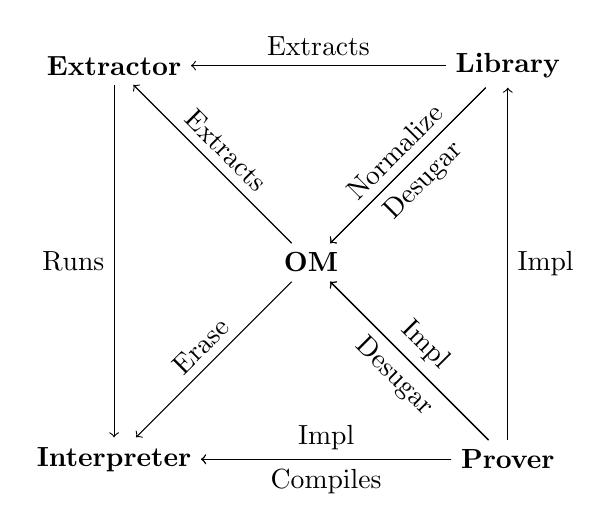
\begin{tikzpicture}
\tikzstyle{every initial by arrow}=[]
    \node (a) at (0,0) {\bf Interpreter};
    \node (b) at (0,5) {\bf Extractor};
    \node (c) at (5,0) {\bf Prover};
    \node (d) at (5,5) {\bf Library};
    \node (e) at (2.5,2.5) {\bf OM};
    \draw [->] (b) to node [left] {Runs} (a);
    \draw [->] (c) to node [below] {Compiles} (a);
    \draw [->] (c) to node [above] {Impl} (a);
    \draw [->] (e) to node [above,sloped] {Erase} (a);
    \draw [->] (d) to node [above,sloped] {Normalize} (e);
    \draw [->] (d) to node [below,sloped] {Desugar} (e);
    \draw [->] (d) to node [above] {Extracts} (b);
    \draw [->] (c) to node [right] {Impl} (d);
    \draw [->] (e) to node [above,sloped] {Extracts} (b);
    \draw [->] (c) to node [below,sloped] {Desugar} (e);
    \draw [->] (c) to node [above,sloped] {Impl} (e);
\end{tikzpicture}
\end{center}
